\chapter{Les tableaux}
\label{les-tableaux}

Poursuivons notre tour d'horizon des données complexes avec
les \textbf{tableaux}.

Comme les structures, les tableaux sont des regoupements de plusieurs
objets. Cependant, à l'inverse de celles-ci, les tableaux regroupe des
données de \emph{même type} et de manière \emph{contiguë} (ce qui exclut
la présence de multiplets de bourrage).

\begin{figure}[htbp]
\centering
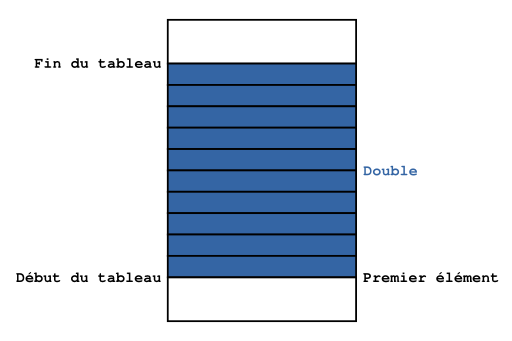
\includegraphics[scale=0.5]{images/tableau_memoire.png}
\caption{Représentation d'un tableau en mémoire}
\end{figure}

Un tableau est donc un gros bloc de mémoire de \emph{taille finie} qui
commence à une adresse déterminée : celle de son premier élément.

\section{Les tableaux simples (à une dimension)}
\label{les-tableaux-simples-(a-une-dimension}

\subsection{Définition}
\label{definition-1}

La définition d'un tableau nécessite trois informations :

\begin{itemize}
\item
  le type des éléments du tableau (rappelez-vous : un tableau est une
  suite de données de \emph{même type}) ;\\
\item
  le nom du tableau (en d'autres mots, son identificateur) ;\\
\item
  \textbf{la longueur} du tableau (le nombre d'éléments qui le
  composent). Cette dernière doit \emph{obligatoirement} être une
  constante entière.
\end{itemize}

\begin{C}
type identificateur[longueur];
\end{C}

Comme vous le voyez, la syntaxe de la déclaration d'un tableau est
similaire à celle d'une variable, la seule différence étant qu'il vous
est nécessaire de préciser le nombre d'éléments entre crochets à la
suite de l'identificateur du tableau.

Ainsi, si nous souhaitons par exemple définir un tableau contenant vingt
\mybox{int}, nous devons procéder comme suit.

\begin{C}
int tab[20];
\end{C}

\subsection{Initialisation}
\label{initialisation-4}

Comme pour les variables, il est possible d'initialiser un tableau ou,
plus précisément, tout ou partie de ses éléments.

\subsubsection{Initialisation avec une longueur explicite}
\label{initialisation-avec-une-longueur-explicite-1}

L'initialisation se réalise de la même manière que pour les structures,
c'est-à-dire à l'aide d'une liste d'initialisation.

\begin{C}
int tab[3] = { 1, 2, 3 };
\end{C}

L'exemple ci-dessus initialise les trois membres du tableau avec les
valeurs 1, 2 et 3.

\begin{attentionbox}
  Comme pour les structures, dans le cas
où vous ne fournissez pas un nombre suffisant de valeurs, les éléments
oubliés seront initialisés à zéro ou, s'il s'agit de pointeurs, seront
des pointeurs nuls.
\end{attentionbox}


Pour un tableau de structures, la liste d'initialisation comportera
elle-même une liste d'initialistation pour chaque structure composant le
tableau.

\begin{C}
struct temps tab[2] = { { 12, 45, 50.6401 }, { 13, 30, 35.480 } } ;
\end{C}

\begin{infobox}
 Notez que, inversément, une structure
peut comporter des tableaux comme membres.
\end{infobox}


\subsubsection{Initialisation avec une longueur implicite}
\label{initialisation-avec-une-longueur-implicite-1}

Lorsque vous initialisez un tableau, il vous est permis d'omettre la
longueur de celui-ci, car le compilateur sera capable d'en déterminer la
taille en comptant le nombre d'éléments présents dans la liste
d'initialisation. Ainsi, l'exemple ci-dessous est correct et défini un
tableau de trois \mybox{int} valant respectivement 1, 2 et 3.

\begin{C}
int tab[] = { 1, 2, 3 };
\end{C}

\subsection{Accès aux éléments d'un tableau}
\label{acces-aux-elements-dun-tableau}

L'accès aux éléments d'un tableau se réalise à l'aide d'un
\textbf{indice}, un nombre entier correspondant à la position de chaque
élément dans le tableau (premier, deuxième, troisième, etc). Cependant,
il y a une petite subtilité : \emph{les indices commencent toujours à
zéro}.

Ceci tient au fait que l'accès aux différents éléments est réalisé à
l'aide de l'adresse du premier élément à laquelle est ajouté l'indice
(qui doit donc être nul pour conserver l'adresse du premier élément).
Étant donné que tous les éléments ont la même taille et se suivent en
mémoire, leurs adresses peuvent effectivement se calculer à l'aide de
l'adresse du premier élément et d'un décalage par rapport à celle-ci
(l'indice, donc).

Prenons un exemple avec un tableau composés de \mybox{int} (ayant une
taille de quatre octets) et dont le premier élément est placé à
l'adresse 1008. Si vous déterminez à la main les adresses de chaque
élèment, vous obtiendrez ceci.

\begin{table}
\centering
\rowcolors{1}{gris-clair-tab}{}
\begin{tabular}{|l|l|}\hline
\rowcolor{gris-tab-entete}\textbf{\makecell{Indice}} & A\textbf{\makecell{dresse de l'élément}}\tabularnewline\hline
0 & 1008 (1008 + 0)\tabularnewline\hline
1 & 1012 (1008 + 4)\tabularnewline\hline
2 & 1016 (1008 + 8)\tabularnewline\hline
3 & 1020 (1008 + 12)\tabularnewline\hline
4 & 1024 (1008 + 16)\tabularnewline\hline
5 & 1028 (1008 + 20)\tabularnewline\hline
\ldots{} & \ldots{}\tabularnewline\hline
\end{tabular}
\end{table}

En fait, il est possible de reformuler ceci à l'aide d'une
multiplication entre l'indice et la taille d'un \mybox{int}.

\begin{table}
\centering
\rowcolors{1}{gris-clair-tab}{}
\begin{tabular}{|l|l|}\hline
\rowcolor{gris-tab-entete}\textbf{\makecell{Indice}} & \textbf{\makecell{Adresse de l'élément}}\tabularnewline\hline
0 & 1008 (1008 + (0 * 4))\tabularnewline\hline
1 & 1012 (1008 + (1 * 4))\tabularnewline\hline
2 & 1016 (1008 + (2 * 4))\tabularnewline\hline
3 & 1020 (1008 + (3 * 4))\tabularnewline\hline
4 & 1024 (1008 + (4 * 4))\tabularnewline\hline
5 & 1028 (1008 + (5 * 4))\tabularnewline\hline
\ldots{} & \ldots{}\tabularnewline\hline
\end{tabular}
\end{table}

Nous pouvons désormais formaliser mathématiquement tout ceci en posant
\(T\) la taille d'un élément du tableau, \(i\) l'indice de cet élément,
et \(A\) l'adresse de début du tableau (l'adresse du premier élément,
donc). L'adresse de l'élément d'indice \(i\) s'obtient en calculant
\(A + T \times i\). Ceci étant posé, voyons à présent comment mettre
tout cela en œuvre en C.

\subsubsection{Le premier élément}
\label{le-premier-element}

Pour commencer, nous avons besoin de l'adresse du premier élément du
tableau. Celle-ci s'obtient en fait d'une manière plutôt
contre-intuitive : lorsque vous utilisez une variable de type tableau
dans une expression, celle-ci est convertie implicitement en un pointeur
\emph{constant} sur son premier élément. Comme vous pouvez le constater
dans l'exemple qui suit, nous pouvons utiliser la variable \mybox{tab}
comme nous l'aurions fait s'il s'agissait d'un pointeur.

\begin{C}
#include <stdio.h>

int main(void)
{
    int tab[3] = { 1, 2, 3 };

    printf("Premier élément : %d\n", *tab);
    return 0;
}
\end{C}

\begin{C}
Premier élément : 1
\end{C}

Notez que comme il s'agit d'une conversion implicite vers un pointeur
constant, il n'est pas possible d'affecter une valeur à une variable de
type tableau. Ainsi, le code suivant est incorrect.

\begin{C}
int t1[3];
int t2[3];

t1 = t2; /* Incorrect. */
\end{C}

La règle de conversion implicite comprends néanmoins deux exceptions :
l'opérateur \mybox{\&} et l'opérateur \mybox{sizeof}.

Lorsqu'il est appliqué à une variable de type tableau, l'opérateur
\mybox{\&} produit comme résultat l'adresse du premier élément du
tableau. Si vous exécutez le code ci-dessous, vous constaterez que les
deux expressions donnent un résultat identique.

\begin{C}
#include <stdio.h>


int main(void)
{
    int tab[3];

    printf("%p == %p\n", (void *)tab, (void *)&tab);
    return 0;
}
\end{C}

Dans le cas où une expression de type tableau est fournie comme opérande
de l'opérateur \mybox{sizeof}, le résultat de celui-ci sera bien la
taille totale du tableau (en multiplets) et non la taille d'un pointeur.

\begin{C}
 #include <stdio.h>


int main(void)
{
    int tab[3];
    int *ptr;

    printf("sizeof tab = %u\n", (unsigned)sizeof tab);
    printf("sizeof ptr = %u\n", (unsigned)sizeof ptr);
    return 0;
}
\end{C}



\begin{C}
sizeof tab = 12
sizeof ptr = 8
\end{C}

Cette propriété vous permet d'obtenir le nombre d'éléments d'un tableau
à l'aide de l'expression suivante.

\begin{C}
sizeof tab / sizeof tab[0]
\end{C}

\subsubsection{Les autres éléments}
\label{les-autres-elements}

Pour accéder aux autres éléments, il va nous falloir ajouter la position
de l'élément voulu à l'adresse du premier élément et ensuite utiliser
l'adresse obtenue. Toutefois, recourir à la formule présentée au-dessus
ne marchera pas car, en C, les pointeurs sont typés. Dès lors, lorsque
vous additionnez un nombre à un pointeur, le compilateur multiplie
automatiquement ce nombre par la taille du type d'objet référencé par le
pointeur. Ainsi, pour un tableau de \mybox{int}, l'expression
\mybox{tab\ +\ 1} est implicitement convertie en
\mybox{tab\ +\ sizeof(int)}.

Voici un exemple affichant la valeur de tous les éléments d'un tableau.

\begin{C}
#include <stdio.h>


int main(void)
{
    int tab[3] = { 1, 2, 3 };

    printf("Premier élément : %d\n", *tab);
    printf("Deuxième élément : %d\n", *(tab + 1));
    printf("Troisième élément : %d\n", *(tab + 2));
    return 0;
}
\end{C}

\begin{C}
Premier élément : 1
Deuxième élément : 2
Troisième élément : 3
\end{C}

L'expression \mybox{*(tab\ +\ i)} étant quelque peu lourde, il existe
un opérateur plus concis pour réaliser cette opération : l'opérateur
\mybox{{[}{]}}. Celui-ci s'utilise de cette manière.

\begin{C}
expression[indice]
\end{C}

Ce qui est équivalent à l'expression suivante.

\begin{C}
*(expression + indice)
\end{C}

L'exemple suivant est donc identique au précédent.

\begin{C}
#include <stdio.h>


int main(void)
{
    int tab[3] = { 1, 2, 3 };

    printf("Premier élément : %d\n", tab[0]);
    printf("Deuxième élément : %d\n", tab[1]);
    printf("Troisième élément : %d\n", tab[2]);
    return 0;
}
\end{C}

\subsection{Parcours et débordement}
\label{parcours-et-debordement}

Une des erreurs les plus fréquente en C consiste à dépasser la taille
d'un tableau, ce qui est appelé un cas de \textbf{débordement}
(\emph{overflow} en anglais). En effet, si vous tentez d'accéder à un
objet qui ne fait pas partie de votre tableau, vous réalisez un accès
mémoire non autorisé, ce qui provoquera un comportement indéfini. Cela
arrive généralement lors d'un parcours de tableau à l'aide d'une boucle.

\begin{C}
#include <stdio.h>


int main(void)
{
    int tableau[5] = {784, 5, 45, -12001, 8};
    int somme = 0;
    unsigned i; 

    for (i = 0; i <= 5; ++i)
        somme += tableau[i];

    printf("%d\n", somme);
    return 0;
}
\end{C}

Le code ci-dessus est volontairement erroné et tente d'accéder à un
élément qui se situe au-delà du tableau. Ceci provient de l'utilisation
de l'opérateur \mybox{\textless{}=} à la place de l'opérateur
\mybox{\textless{}} ce qui entraîne un tour de boucle avec \mybox{i}
qui est égal à 5, alors que le dernier indice du tableau doit être
quatre.

\begin{attentionbox}
  N'oubliez pas : les indices d'un
tableau commencent \emph{toujours} à zéro. En conséquence, les indices
valides d'un tableau de \(n\) éléments vont de 0 à \(n-1\).
\end{attentionbox}


\subsection{Tableaux et fonctions}
\label{tableaux-et-fonctions}

\subsubsection{Passage en argument}
\label{passage-en-argument-1}

Étant donné qu'un tableau peut être utilisé comme un pointeur sur son
premier élément, lorsque vous passer un tableau en argument d'une
fonction, celle-ci reçoit un pointeur vers le premier élément du
tableau. Le plus souvent, il vous sera nécessaire de passer également la
taille du tableau afin de pouvoir le parcourir.

Le code suivante utilise une fonction pour parcourir un tableau d'entier
et afficher la valeur de chacun de ses éléments.

\begin{C}
#include <stdio.h>


void affiche_tableau(int *tab, unsigned taille)
{
    unsigned i;

    for (i = 0; i < taille; ++i)
        printf("tab[%u] = %d\n", i, tab[i]);
}


int main(void)
{
    int tab[5] = { 2, 45, 67, 89, 123 };

    affiche_tableau(tab, 5);
    return 0;
}
\end{C}

\begin{C}
tab[0] = 2
tab[1] = 45
tab[2] = 67
tab[3] = 89
tab[4] = 123
\end{C}

\begin{infobox}
Notez qu'il existe une syntaxe
alternative pour déclarer un paramètre de type tableau héritée du
langage B (voyez la dernière section)

\begin{C}
 void affiche_tableau(int tab[], unsigned taille)
\end{C}

Toutefois, nous vous conseillons de recourir à la
première écriture, cette dernière étant plus explicite.
\end{infobox}

\subsubsection{Retour de fonction}
\label{retour-de-fonction-1}

De la même manière que pour le passage en argument, retourner un tableau
revient à retourner un pointeur sur le premier élément de celui-ci.
Toutefois, n'oubliez pas les problématiques de classe de stockage ! Si
vous retournez un tableau de classe de stockage automatique, vous
fournissez à la fonction appelante un pointeur vers un objet qui
n'existe plus (puisque l'exécution de la fonction appelée est terminée).

\begin{C}
 #include <stdio.h>


int *tableau(void)
{
    int tab[5] = { 1, 2, 3, 4, 5 };

    return tab;
}


int main(void)
{
    int *p = tableau(); /* Incorrect. */

    printf("%d\n", p[0]);
    return 0;
}
\end{C}

\section{La vérité sur les tableaux }
\label{la-verite-sur-les-tableaux }

Nous vous avons dit qu'une variable de type tableau pouvait être
utilisée comme un pointeur constant sur son premier élément. Cependant,
ce n'est pas tout à fait vrai.

\subsection{Un peu d'histoire}
\label{un-peu-dhistoire}

Le prédécesseur du langage C était le langage B. Lorsque le
développement du C a commencé, un des objectifs était de le rendre
autant que possible compatible avec le B, afin de ne pas devoir (trop)
modifier les codes existants (un code écrit en B pourrait ainsi être
compilé avec un compilateur C sans ou avec peu de modifications). Or, en
B, un tableau se définissait comme suit.

\begin{C}
auto tab[3];
\end{C}

\begin{infobox}
Le langage B était un langage non
typé, ce qui explique l'absence de type dans la définition. Le mot-clé
\mybox{auto} (toujours présent en langage C, mais devenu obsolète)
servait à indiquer que la variable définie était de classe de stockage
automatique.
\end{infobox}


Toutefois, à la différence du langage C, cette définition créée un
tableau de trois éléments \emph{et} un pointeur initialisé avec
l'adresse du premier élément. Ainsi, pour créer un pointeur, il
suffisait de définir une variable comme un tableau de taille nulle.

\begin{C}
auto ptr[];
\end{C}

Le langage C, toujours en gestation, avait repris ce mode de
fonctionnement. Cependant, les structures sont arrivées et les problèmes
avec. En effet, prenez ce bout de code.

\begin{C}
#include <stdio.h>

struct exemple {
    int tab[3];
};


struct exemple exemple_init(void)
{
    struct exemple init = { { 1, 2, 3 } };

    return init;
}


int main(void)
{
    struct exemple s = exemple_init();

    printf("%d\n", s.tab[0]);
    return 0;
}
\end{C}

La fonction \mybox{exemple\_init()} retourne une structure qui est
utilisée pour initialiser la variable de la fonction \mybox{main()}.
Dans un tel cas, comme pour n'importe quelle variable, le contenu de la
première structure sera intégralement copié dans la deuxième. Le souci,
c'est que si une définition de tableau créer un tableau \emph{et} un
pointeur initialisé avec l'adresse du premier élément de celui-ci, alors
il est nécessaire de modifier le champ \mybox{tab} de la structure
\mybox{s} lors de la copie sans quoi son champ \mybox{tab} pointera
vers le tableau de la structure \mybox{init} (qui n'existera plus
puisque de classe de stockage automatique) et non vers le sien. Voilà
qui complexifie la copie de structures, particulièrement si sa
définition comprend plusieurs tableaux possiblement imbriqués\ldots{}

Pour contourner ce problème, les concepteurs du langage C ont imaginé
une solution (tordue) qui est à l'origine d'une certaine confusion dans
l'utilisation des tableaux : une variable de type tableau \emph{ne sera
plus un pointeur}, mais sera \emph{convertie en un pointeur sur son
premier élément lors de son utilisation}.

\subsection{Conséquences de l'absence d'un pointeur}
\label{consequences-de-labsence-dun-pointeur}

Étant donné qu'il n'y a plus de pointeur alloué, la copie de structures
s'en trouve simplifiée et peut être réalisée sans opération particulière
(ce qui était l'objectif recherché).

Toutefois, cela entraîne une autre conséquence : il n'est plus possible
d'assigner une valeur à une variable de type tableau, seuls ses éléments
peuvent se voir affecter une valeur. Ainsi, le code suivant est
incorrect puisqu'il n'y a aucun pointeur pour recevoir l'adresse du
premier élément du tableau \mybox{t2}.

\begin{C}
int t1[3];
int t2[3];

t1 = t2; /* Incorrect. */
\end{C}

Également, puisqu'une variable de type tableau n'est plus un pointeur,
celle-ci n'a pas d'adresse. Dès lors, lorsque l'opérateur \mybox{\&}
est appliqué à une variable de type tableau, le résultat sera l'adresse
du premier élément du tableau puisque seuls les éléments du tableau ont
une adresse.

\section{Les tableaux multidimensionnels}
\label{les-tableaux-multidimensionnels}

Jusqu'à présent, nous avons travaillés avec des tableaux linéaires,
c'est-à-dire dont les éléments se suivaient les uns à la suite des
autres. Il s'agit de tableaux dit à une dimension ou
\textbf{unidimensionnels}.

Cependant, certaines données peuvent être représentées plus simplement
sous la forme de tableaux à deux dimensions (autrement dit, organisées
en lignes et en colonnes). C'est par exemple le cas des images (non
vectorielles) qui sont des matrices de pixels ou, plus simplement, d'une
grille de Sudoku qui est organisée en neuf lignes et en neuf colonnes.

Le langage C vous permet de créer et de gérer ce type de tableaux dit
\textbf{multidimensionnels} (en fait, des tableaux de tableaux) et ce,
bien au-delà de deux dimensions.

\subsection{Définition}
\label{definition-2}

La définition d'un tableau multidimensionnel se réalise de la même
manière que celle d'un tableau unidimensionnel si ce n'est que vous
devez fournir la taille des différentes dimensions.

Par exemple, si nous souhaitons définir un tableau de \mybox{int} de
vingt lignes et trente-cinq colonnes, nous procèderons comme suit.

\begin{C}
int tab[20][35];
\end{C}

De même, pour un tableau de \mybox{double} à trois dimensions.

\begin{C}
double tab[3][4][5];
\end{C}

\section{Initialisation}
\label{initialisation-5}

\subsection{Initialisation avec une longueur explicite}
\label{initialisation-avec-une-longueur-explicite-2}

Comme pour les tableaux de structures, l'initialisation d'un tableau
multidimensionnel s'effectue à l'aide d'une liste d'initialisation
comprenant elle-même des listes d'initialisations.

\begin{C}
int t1[2][2] = { { 1, 2 }, { 3, 4 } };
int t2[2][2][2] = { { { 1, 2 }, { 3, 4 } }, { { 5, 6 }, { 7, 8 } } };
\end{C}

\begin{attentionbox}
 Comme pour les tableaux
unidimensionnel, dans le cas où vous ne fournissez pas un nombre
suffisant de valeurs, les éléments omis seront initialisés à zéro ou,
s'il s'agit de pointeurs, seront des pointeurs nuls.
\end{attentionbox}


\subsection{Initialisation avec une longueur implicite}
\label{initialisation-avec-une-longueur-implicite-2}

Lorsque vous initialisez un tableau multidimensionnel, il vous est
permis d'omettre la taille de la \emph{première dimension}. La taille
des autres dimensions doit en revanche être spécifiée, le compilateur ne
pouvant déduire la taille de toutes les dimensions.

\begin{C}
int t1[][2] = { { 1, 2 }, { 3, 4 } };
int t2[][2][2] = { { { 1, 2 }, { 3, 4 } }, { { 5, 6 }, { 7, 8 } } };
\end{C}

\subsection{Utilisation}
\label{utilisation-4}

Techniquement, un tableau multidimensionnel est un tableau dont les
éléments sont eux-mêmes des tableaux. Dès lors, vous avez besoin
d'autant d'indices qu'il y a de dimensions. Par exemple, pour un tableau
à deux dimensions, vous avez besoin d'un premier indice pour accéder à
l'élément souhaité du premier tableau, mais comme cet élément est
lui-même un tableau, vous devez utiliser un second indice pour
sélectionner un élément de celui-ci. Illustration.

\begin{C}
#include <stdio.h>


int main(void)
{
    int tab[2][2] = { { 1, 2 }, { 3, 4 } };

    printf("tab[0][0] = %d\n", tab[0][0]);
    printf("tab[0][1] = %d\n", tab[0][1]);
    printf("tab[1][0] = %d\n", tab[1][0]);
    printf("tab[1][1] = %d\n", tab[1][1]);
    return 0;
}
\end{C}

\begin{C}
tab[0][0] = 1
tab[0][1] = 2
tab[1][0] = 3
tab[1][1] = 4
\end{C}

\subsection{Représentation en mémoire}
\label{representation-en-memoire-1 }

Techniquement, les données d'un tableau multidimensionnel sont stockées
les unes à coté des autres en mémoire : elles sont rassemblées dans un
tableau à une seule dimension. Si les langages comme le FORTRAN
mémorisent les colonnes les unes après les autres (\emph{column-major
order} en anglais), le C mémorise les tableaux lignes par lignes
(\emph{row-major order}).

\begin{figure}[htbp]
\centering
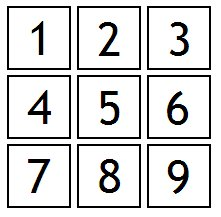
\includegraphics[scale=0.5]{images/tableau_2_dimension.jpg}
\caption{Exemple de tableau en deux dimensions}
\end{figure}

\begin{figure}[htbp]
\centering
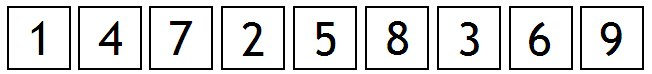
\includegraphics[scale=0.5]{images/column_major_order.jpg}
\caption{Column-major order}
\end{figure}

\begin{figure}[htbp]
\centering
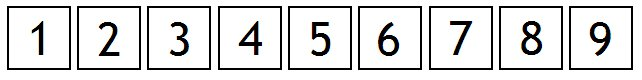
\includegraphics[scale=0.5]{images/row_major_order.jpg}
\caption{Row-major order}
\end{figure}

Le calcul d'adresse à effectuer est une généralisation du calcul vu au
chapitre précédent.

\subsection{Parcours}
\label{parcours}

Le même exemple peut être réalisé à l'aide de deux boucles imbriquées
afin de parcourir le tableau.

\begin{C}
#include <stdio.h>


int main(void)
{
    int tab[2][2] = { { 1, 2 }, { 3, 4 } };
    unsigned i;
    unsigned j;

    for (i = 0; i < 2; ++i)
        for (j = 0; j < 2; ++j)
            printf("tab[%u][%u] = %d\n", i, j, tab[i][j]);

    return 0;
}
\end{C}

\subsection{Tableaux multidimensionnels et fonctions}
\label{tableaux-multidimensionnels-et-fonctions}

\subsubsection{Passage en argument}
\label{passage-en-argument}

Souvenez-vous : sauf exceptions, un tableau est converti en un pointeur
sur son premier élément. Dès lors, qu'obtenons-nous lors du passage d'un
tableau à deux dimensions en argument d'une fonction ? Le premier
élément du tableau est un tableau, donc un pointeur sur\ldots{} Un
tableau (\emph{hé} oui). :p

La syntaxe d'un pointeur sur tableau est la suivante.

\begin{C}
type (*identificateur)[taille];
\end{C}

Vous remarquerez la présence de parenthèses autour du symbole \mybox{*}
et de l'identificateur afin de signaler au compilateur qu'il s'agit d'un
pointeur sur un tableau et non d'un tableau de pointeurs. Également,
notez que la taille du tableau référencé doit être spécifiée. En effet,
sans celle-ci, le compilateur ne pourrait pas opérer correctement le
calcul d'adresses puisqu'il ne connaîtrait pas la taille des éléments
composant le tableau référencé par le pointeur.

La même logique peut-être appliquée pour créer des pointeur sur des
tableaux de tableaux.

\begin{C}
type (*identificateur)[N][M];
\end{C}

Et ainsi de suite jusqu'à ce que mort s'en suive\ldots{} :-°

L'exemple ci-dessous illustre ce qui vient d'être dit en utilisant une
fonction pour afficher le contenu d'un tableau à deux dimensions de
\mybox{int}.

\begin{C}
#include <stdio.h>


void affiche_tableau(int (*tab)[2], unsigned n, unsigned m)
{
    unsigned i;
    unsigned j;

    for (i = 0; i < n; ++i)
        for (j = 0; j < m; ++j)
            printf("tab[%u][%u] = %d\n", i, j, tab[i][j]);
}


int main(void)
{
    int tab[2][2] = { { 1, 2 }, { 3, 4 } };

    affiche_tableau(tab, 2, 2);
    return 0;
}
\end{C}

\subsubsection{Retour de fonction}
\label{retour-de-fonction-2}

Même remarque que pour les tableaux unidimensionnels : attention à la
classe de stockage ! Pour le reste, nous vous laissons admirer la
syntaxe particulièrement dégoûtante d'une fonction retournant un
pointeur sur un tableau de deux \mybox{int}.

\begin{C}
 #include <stdio.h>


int (*tableau(void))[2] /* Ouh ! Que c'est laid ! */
{
    int tab[2][2] = { { 1, 2 }, { 3, 4 } };

    return tab;
}


int main(void)
{
    int (*p)[2] = tableau(); /* Incorrect. */

    printf("%d\n", p[0][0]);
    return 0;
}
\end{C}

\section{Exercices}
\label{exercices-4}

\subsection{Somme des éléments}
\label{somme-des-elements}

Réalisez une fonction qui calcule la somme de tous les éléments d'un
tableau de \mybox{int}.

\begin{C}
 int somme(int *tab, unsigned taille)
{
    unsigned i;
    int res = 0 ;

    for (i = 0; i < taille; ++i)
        res += tableau[i];

    return res;
}
\end{C}

\subsection{Maximum et minimum}
\label{maximum-et-minimum}

Créez deux fonctions : une qui retourne le plus petit élément d'un
tableau de \mybox{int} et une qui renvoie le plus grand élément d'un
tableau de \mybox{int}.

\begin{C}
 int minimum(int *tab, unsigned taille)
{
    unsigned i;
    int min = tab[0];

    for (i = 1; i < taille; ++i)
        if (tab[i] < min)
            min = tab[i];

    return min;
}


int maximum(int *tab, unsigned taille)
{
    unsigned i;
    int max = tab[0];

    for (i = 1; i < taille; ++i)
        if (tab[i] > max)
            max = tab[i];

    return max
}
\end{C}

\subsection{Recherche d'un élément}
\label{recherche-dun-element}

Construisez une fonction qui teste la présence d'une valeur dans un
tableau de \mybox{int}. Celle-ci retournera 1 si un ou plusieurs
éléments du tableau sont égaux à la valeur recherchée, 0 sinon.

\begin{C}
 int find(int * tab, unsigned taille, int val)
{
    unsigned i;

    for (i = 0; i < taille; ++i)
        if (tab[i] == val) 
            return 1;

    return 0;
}
\end{C}

\subsection{Inverser un tableau}
\label{inverser-un-tableau}

Produisez une fonction qui inverse le contenu d'un tableau (le premier
élément devient le dernier, l'avant dernier le deuxième et ainsi de
suite).

\subsubsection{Indice}
\label{indice}

\begin{secretbox}
  Pensez à la fonction \mybox{swap()}
présentée dans le chapitre sur les pointeurs.
\end{secretbox}


\subsubsection{Correction}
\label{correction-16}

\begin{C}
 void swap(int *pa, int *pb)
{
    int tmp;

    tmp = *pa;
    *pa = *pb;
    *pb = tmp;
}


void invert(int *tab , unsigned taille)
{
    unsigned i;

    for (i = 0; i < (taille / 2); ++i)
        swap(tab + i , tab + taille - 1 - i);
    }
}
\end{C}

\subsection{Produit des lignes}
\label{produit-des-lignes}

Composez une fonction qui calcul le produit de la somme des éléments de
chaque ligne d'un tableau de \mybox{int} à deux dimensions (ce tableau
comprend cinq lignes et cinq colonnes).

\begin{C}
 int produit(int (*tab)[5])
{
    unsigned i;
    unsigned j;
    int res = 1;

    for (i = 0; i < 5; ++i)
    {
        int tmp = 0;

        for (j = 0; j < 5; ++j)
            tmp += tab[i][j];

        res *= tmp;
    }

    return res;
}
\end{C}

\subsection{Triangle de Pascal}
\label{triangle-de-pascal}

Les triangles de Pascal sont des objets mathématiques amusants. Voici
une petite animation qui vous expliquera le fonctionnement de ceux-ci.

\begin{figure}[htbp]
\centering
\includegraphics[scale=0.5]{images/PascalTriangleAnimated2-0.png}
%\animategraphics[autoplay,loop]{8}{images/PascalTriangleAnimated2-}{0}{97}
\caption{Explication des triangles de Pascal en image}
\end{figure}

Votre objectif va être de réaliser un programme qui affiche un triangle
de Pascal de la taille souhaitée par l'utilisateur. Pour ce faire, nous
allons diviser le triangle en lignes afin de pouvoir le représenter sous
la forme d'un tableau à deux dimensions. Chaque élément du tableau se
verra attribué soit une valeur du triangle soit zéro pour signaler qu'il
n'est pas utilisé.

La première chose que nous allons faire est donc définir un tableau à
deux dimensions (nous fixerons la taille des dimensions à dix) dont tous
les éléments sont initialisés à zéro. Ensuite, nous allons demandés à
l'utilisateur d'entrer la taille du triangle qu'il souhaite obtenir
(celle-ci ne devra pas être supérieure aux dimensions du tableau).

À présent, passons à la fonction de création du triangle de Pascal.
Celle-ci devra mettre en œuvre l'algorithme suivant.

\begin{C}
N = taille du triangle de Pascal fournie par l’utilisateur

Mettre la première case du tableau à 1

Pour i = 1, i < N, i = i + 1
    Mettre la première case de la ligne à 1

    Pour j = 1, j < i, j = j + 1
         La case [i,j] prend la valeur [i - 1, j - 1] + [i - 1, j]

    Mettre la dernière case de la ligne à 1
\end{C}

Enfin, il vous faudra écrire une petite fonction pour afficher le
tableau ainsi créer.
Bon courage !

\begin{C}
 #include <stdio.h>
#include <stdlib.h>


void triangle_pascal(int (*tab)[10], unsigned taille)
{
    unsigned i;
    unsigned j;

    tab[0][0] = 1;

    for (i = 1; i < taille; ++i)
    {
        tab[i][0] = 1;

        for (j = 1; j < i; ++j)
            tab[i][j] = tab[i - 1][j - 1] + tab[i - 1][j];

        tab[i][i] = 1;
    }
}


void print_triangle(int (*tab)[10], unsigned taille)
{
    unsigned i;
    unsigned j;
    int sp;

    for (i = 0; i < taille; ++i)
    {
        for (sp = taille - 1 - i; sp > 0; --sp)
            printf(" ");

        for (j = 0; j < taille; ++j)
            if (tab[i][j] != 0)
                printf("%d ", tab[i][j]);

        printf("\n");
    }
}


int main(void)
{
    int tab[10][10] = { { 0 } };
    unsigned taille;

    printf("Taille du triangle: ");

    if (scanf("%u", &taille) != 1)
    {
        printf("Mauvaise saisie\n");
        return EXIT_FAILURE;
    }
    else if (taille > 10)
    {
        printf("La taille ne doit pas être supérieure à 10\n");
        return EXIT_FAILURE;
    }

    triangle_pascal(tab, taille);
    print_triangle(tab, taille);  
    return 0;
}
\end{C}

\hrulefill

Dans le chapitre suivant, nous aborderons un nouveau type
d'agrégat, un peu particulier puisqu'il se base sur les tableaux : les
\textbf{chaînes de caractères}.